%%%%%%%%%%%%%%%%%%%%%%%%%%%%%%%%%%%%%%%%%%%%%%%%%%%%%%%%%%
%%%%%%%%%%%%%%%%%% M A K R O S %%%%%%%%%%%%%%%%%%%%%%%%%%%
%%%%%%%%%%%%%%%%%%%%%%%%%%%%%%%%%%%%%%%%%%%%%%%%%%%%%%%%%%

%%%%%%%%%%%%%%%%%%%%%%%% g e n e r e l l e   M a k r o s %%%%%%%%%%%%%%%%%%%%%%%

%% 2019-07-26
%% phi@freimann.eu
%% Makros for BBW-Tex Documents
\usepackage{inputs/bbwColors}

%%%%%%%%%%%%%%%%%% I N C L U D E S   &   I N D E X  %%%%%
\graphicspath{{../img/}}
\graphicspath{{./img/}}

\newcommand\bbwGraphicRaise[3]{\raisebox{#1}{\includegraphics[width=#2]{#3}}}%%
\newcommand\bbwGraphic[2]{\bbwGraphicRaise{-5mm}{#1}{#2}}%%
\newcommand\bbwCenterGraphicRaise[3]{\begin{center}\bbwGraphicRaise{#1}{#2}{#3}\end{center}}
\newcommand\bbwCenterGraphic[2]{\bbwCenterGraphicRaise{-5mm}{#1}{#2}}%%


%% All in one Skript
\newif\ifisALLINONE
\isALLINONEfalse

%% Blended Learning
%% Insb. MatheNinja Links. Diese sind jedoch in einem anderen Kurs!
\newif\ifisBLENDED
\isBLENDEDfalse


%%%%%%%%% TRAINER Version vs. Schülerversion %%%%%%%%%%%%%

\newcommand\TRAINER[1]{%%
{%%
\ifisTRAINER{\color{BlueGreen}{#1}}%%
\fi%%
}}%%  

\newcommand\TALS[1]{%
{%%
\ifisTALS{#1}%%
\fi%%
}}%

\newcommand\GESO[1]{%
{%%
\ifisGESO{#1}%%
\fi%%
}}%    

\newcommand\BLENDED[1]{%
{%%
\ifisBLENDED{#1}%%
\fi%%
}}%    

\newcommand{\noTRAINER}[1]{{\ifisTRAINER{}\else{#1}\fi}{}}%%



%%\makeatletter
%% Je nach Umgebung "environment" wird das mmPapier breiter oder
%% schmaler
%% bei itemize sollen 16.4 und bei definiton-Boxen 16.8 mm genommen
%% werden.


\usepackage{inputs/mmPapierbreiteSty}


%% Trainer "no" Dotfill
%% If no Trainer: Dotfill
\newcommand{\TNDF}[1]{\TRAINER{#1}\noTRAINER{\dotfill{}}}%%

\newcommand{\leserluft}{\vspace{2mm}}

%% Notiz felder 
%% Anwendung:
%% \noteField{10}  
%%  --> Notizfeld mit 10 Leerzeilen
\newcounter{DFCounter}

\newcommand*{\noteField}[1]{%
\setcounter{DFCounter}{1}
\vspace{0.5in}%
\begin{tabular}{p{14cm}}%
\hline%
\vspace{0.2cm}
Notizen: \\%
\whiledo{\theDFCounter < #1}{%
\dotfill \\
\addtocounter{DFCounter}{1}%
}%
\end{tabular}%
}%

\newcommand*{\noteLines}[1]{%
\setcounter{DFCounter}{1}
\vspace{0.1cm}%
\begin{tabular}{p{14cm}}%
\whiledo{\theDFCounter < #1}{%
\dotfill \\
\addtocounter{DFCounter}{1}%
}%
\end{tabular}%
}%

%% Platz für Notizen, aber nur bei Schülernverison (\noTRAINER)
\newcommand{\platzFuerTNNotes}[1]{%
\ifisTRAINER{}\else{%%
Platz für Notizen:\newline%%
\noteLines{#1}%%
}\fi{}%
}%%

%% Vier Leerzeilen für Notizen
\newcommand*\dotfillpara{%
\begin{tabular}{p{11.5cm}}%
\hfill   \\
\dotfill \\
\dotfill \\
\dotfill \\
\dotfill
\end{tabular}%
}


%%Häuschenpapier
\newcommand{\mmPapierZwei}[2]{\begin{tikzpicture}
%%  \draw[step=4mm,bbwMMFarbe,ultra thin]
%%  \draw[step=4mm,bbwMMFarbe,thick]
  \draw[step=4mm,bbwMMFarbe,line width=0.02mm]
  (0, 0) grid ({#2}, {#1});
\end{tikzpicture}}%%


%% millimeterPapier füllen bis Ende Seite
\newcommand{\mmPapierBisEndeSeite}{

\begin{tikzpicture}

\newdimen\spaceleftOnPage
\spaceleftOnPage=\dimexpr\textheight-\pagetotal-14pt\relax

\pgfmathsetmacro{\gridWidth}{\textwidth        - mod(\textwidth,      4mm)      }
\pgfmathsetmacro{\gridHeight}{\spaceleftOnPage - mod(\spaceleftOnPage,4mm) - 4mm}

\draw [step=4mm,bbwMMFarbe,line width=0.02mm] (0,0) grid (\gridWidth pt,\gridHeight pt);
\end{tikzpicture}%%
\newpage%%
}%% END Makro mmPapieBisEndeSeite


%% Standardbreite für Arbeitsblätter und das Theorieheft
%% Wird in bbwPruefung.sty überschrieben, da dort schmaler
\def\defaultTextBreite{17.6}
\def\unitCMWhatElse{cm}%% wird als Breitenangabe für den nächsten command verwendet

%% Verwendung: \bbwCenterGraphic{\defaultTextBreite}{«img url»}
\def\defaultTextBreiteCM{\defaultTextBreite\unitCMWhatElse}
\newcommand{\mmPapier}[1]{\mmPapierZwei{#1}{\defaultTextBreite}}


%% Notizen Berechungen auf Prüfungsblättern
\newcommand{\platzFuerBerechnungen}[1]{\noTRAINER{

Notizen / Berechnungen:

\mmPapier{#1}}}%% end platzFuerBerechnungen

\newcommand{\platzFuerBerechnungenBisEndeSeite}[1]{\noTRAINER{

Notizen / Berechnungen:

\mmPapierBisEndeSeite}}%% end platzFuerBerechnungen



\newcommand{\platzFuerBerechnungenOhneText}[1]{\noTRAINER{

\mmPapier{#1}}}


%% Die Abkürzung z.\,B. von «Zum Beispiel» hat einen verkleinerten Abstand.
\newcommand*\zB{%
z.\,B.
}

%%
%% Auf der Titelseite steht entweder GESO oder TALS.
%% Dies wird gleich mit der Fußnote angegeben.
%% Dieses Kommando sollte im Kommando «\untertitel» eingesetzt werden.
%%
\newcommand*\ausrichtungAufTitelseite{%
\ifisTALS{TALS\noTRAINER{\footnote{TALS «Technik, Architektur und Life Sciences
(Laboranten)»: Ausrichtung technisches Profil}}}%%
\fi%%
\ifisGESO{GESO\noTRAINER{\footnote{GESO: Ausrichtung \textbf{Ge}sundheit und \textbf{So}ziales}}}%%
\fi}%%

%%%%%%%%%%%%%%%%%%%%%% B B W - M a t h e   F a r b c o d e s  %%%%%%%%%%%%%%%%%%%%%%%%%%%%%%555

\newcommand{\rezeptFarbe}{rezeptFarbe}
\newcommand{\definitionFarbe}{definitionFarbe}
\newcommand{\gesetzFarbe}{gesetzFarbe}
\newcommand{\beispielFarbe}{beispielFarbe}
\newcommand{\bemerkungFarbe}{bemerkungFarbe}

%% Falls gewünscht übersteuren
%  \definecolor{xyz}{HTML}{eeff66}
%  \renewcommand{\beispielFarbe}{xyz}
%

%% Theorem-Styles
\newcommand\theoremlayoutdefinition[4]{\newtcbtheorem[number within=section]{#1}{#2}%
   {theorem style=plain,enhanced,colframe=#3!20!white,colback=#3!20!white,
     coltitle=#3!60!black,fonttitle=\upshape\bfseries,
     %%fontupper=\itshape,
    %%drop fuzzy shadow=blue!50!black!50!white,
    terminator sign={:},
    borderline north={0.5mm}{0pt}{#3}, borderline south={0.5mm}{0pt}{#3}
   }{#4}}



%% Farben für rezept, definition und gesetz von Marthale übernommen.
%% Verwendung mit * unterbindet die Nummerierung \begin{gesetz*}{Blah}{xy} ...\end {gesetz*}
\theoremlayoutdefinition{rezept}{Rezept}{\rezeptFarbe}{R}
\theoremlayoutdefinition{definition}{Definition}{\definitionFarbe}{D}
\theoremlayoutdefinition{gesetz}{Gesetz}{\gesetzFarbe}{G}%% was green
\theoremlayoutdefinition{beispiel}{Beispiel}{\beispielFarbe}{B}
\theoremlayoutdefinition{bemerkung}{Bemerkung}{\bemerkungFarbe}{M}

%%
%% Force a blank page, when \newpage does not work
%%
\def\blankpage{%
	\clearpage%
	\null%
	\clearpage}%%

\newcommand{\Lueckentext}[1]{\,\,\noTRAINER{\dotfill}\TRAINER{#1}}


\newcommand{\LoesungsRaumCM}[2]{\,\,\noTRAINER{\underline{\hspace{#1}}}\TRAINER{#2}}

\newcommand{\LoesungsRaum}[1]{\LoesungsRaumCM{30mm}{#1}}
\newcommand{\LoesungsRaumKurz}[1]{\LoesungsRaumCM{15mm}{#1}}
\newcommand{\LoesungsRaumLang}[1]{\LoesungsRaumCM{45mm}{#1}}


%% TI nSpire
\def\tinspire{\texttt{TI-nSpire}}

%% TI 30 Pro Mathprint Button Images
\def\tiprobuttonbreite{10mm}
\def\nspirebuttonbreite{8.6mm}

%%\def\sec{\raisebox{-2mm}{\includegraphics[width=\buttonbreite{}]{img/tiprobuttonimages/2nd.png}}}
\newcommand{\tiprobutton}[1]{\raisebox{-2mm}{\mbox{\,\includegraphics[width=\tiprobuttonbreite{}]{img/tiprobuttonimages/#1.png}\,}}}

\newcommand{\nspirebutton}[1]{\raisebox{-2mm}{\mbox{\,\includegraphics[width=\nspirebuttonbreite{}]{img/nspirebuttonimages/#1.png}\,}}}

%% Counter  für Aufgaben
%% Bei jedem Part wird die Aufgabennummer zurückgesetz auf 1
\newcommand{\bbwPartID}{AA1}
\newcommand{\bbwAufgabenBlockID}{}
\newcounter{bbwAufgabenNummerCounter}[part]
\setcounter{bbwAufgabenNummerCounter}{1}
\newcommand{\bbwAufgabenNummer}{\arabic{bbwAufgabenNummerCounter}}
\newcommand{\nextBbwAufgabenNummer}{\stepcounter{bbwAufgabenNummerCounter}}
\newcommand{\aufgSubLabel}{{\color{blue}\bbwAufgabenNummer. \alph*)}}

%% Benutze außerhalb der bbwAufgabenblöcke folgendes Kommando, um an die
%% nächste Aufgabennummer zu kommen. Dies z. B. wenn ein längerer Text vor der Aufgabe steht,
%% der auch schon diese Bezeichnung erhalten sollte
\newcommand{\bbwActAufgabenNr}{{\color{blue}\bbwAufgabenNummer. {\small[\bbwAufgabenBlockID]}}}


\newenvironment{bbwAufgabenBlock}{%% Begin environment Part:

\bbwActAufgabenNr{}
%%{\color{blue}\bbwAufgabenNummer. {\small[\bbwAufgabenBlockID]}}
\begin{enumerate}[label=\aufgSubLabel]
}%% Ende der Präambel
{%% END Part:
\end{enumerate}
\nextBbwAufgabenNummer
}%% END environment bbwAufgabenBlock

%%%%%%%%%%%%%%%%%%%%%%%%%%%%

%% Weblinks und Mathe Ninja Links

\newcommand{\weblink}[2]{\href{#2}{#1}}

\newcommand{\olatBBWLogo}{
\includegraphics[width=15mm]{logos/traube.pdf}}%%


\newcommand{\olatLOGOLink}[3]{%%
\begin{tabular}{|lp{111mm}|}\hline%%
\weblink{\raisebox{-5mm}{\olatBBWLogo{}}}{#2} & \weblink{#1}{#2}\\
\multicolumn{2}{|p{172mm}|}{\cellcolor{aufgabenFarbe}#3}\\\hline
\end{tabular}%%
}%% END Command olatLOGOLink

%% Use:
%% \olatLinkArbeitsblatt{Kapitel/Arbeitsblattname «[ID]»}{«URL»}{Aufgabennummern}
\newcommand{\olatLinkArbeitsblatt}[3]{\olatLOGOLink{Blatt: #1}{#2}{#3}}%%

%% Use:
%% \olatLinkPruefung{Einstiegstest}{«URL»}
\newcommand{\olatLinkPruefung}[2]{\olatLOGOLink{Online Prüfung}{#2}{#1}}%%

%% Use
%% \olatLinkGESOKompendium{Kapitel}{Seite/Seiteff}{Aufgabe(n)}
\newcommand{\olatLinkGESOKompendium}[3]{\GESO{\olatLOGOLink{Kompendium}{https://olat.bbw.ch/auth/RepositoryEntry/572162163/CourseNode/102901164962365}{Kapitel #1; Seite #2; Aufgaben #3}}}%%


%% Use
%% \olatLinkTALSStrukturaufgaben[SPF|GLF]{«Seite(n)/Aufgabe(n)»}
\newcommand{\olatLinkTALSStrukturaufgabenSPF}[1]{\olatLOGOLink{Strukturaufgaben Schwerpunktsfach}{https://olat.bbw.ch/auth/RepositoryEntry/572162090/CourseNode/102901174299246}{#1}}
\newcommand{\olatLinkTALSStrukturaufgabenGLF}[1]{\olatLOGOLink{Strukturaufgaben Grundlagenfach}{https://olat.bbw.ch/auth/RepositoryEntry/572162090/CourseNode/102901174291476}{#1}}

%%
%% use:
%% \matheNinjaLink{Beschreibung}{URL}
\newcommand{\matheNinjaLink}[2]{\olatLOGOLink{Mathe Ninja Link \raisebox{-6mm}{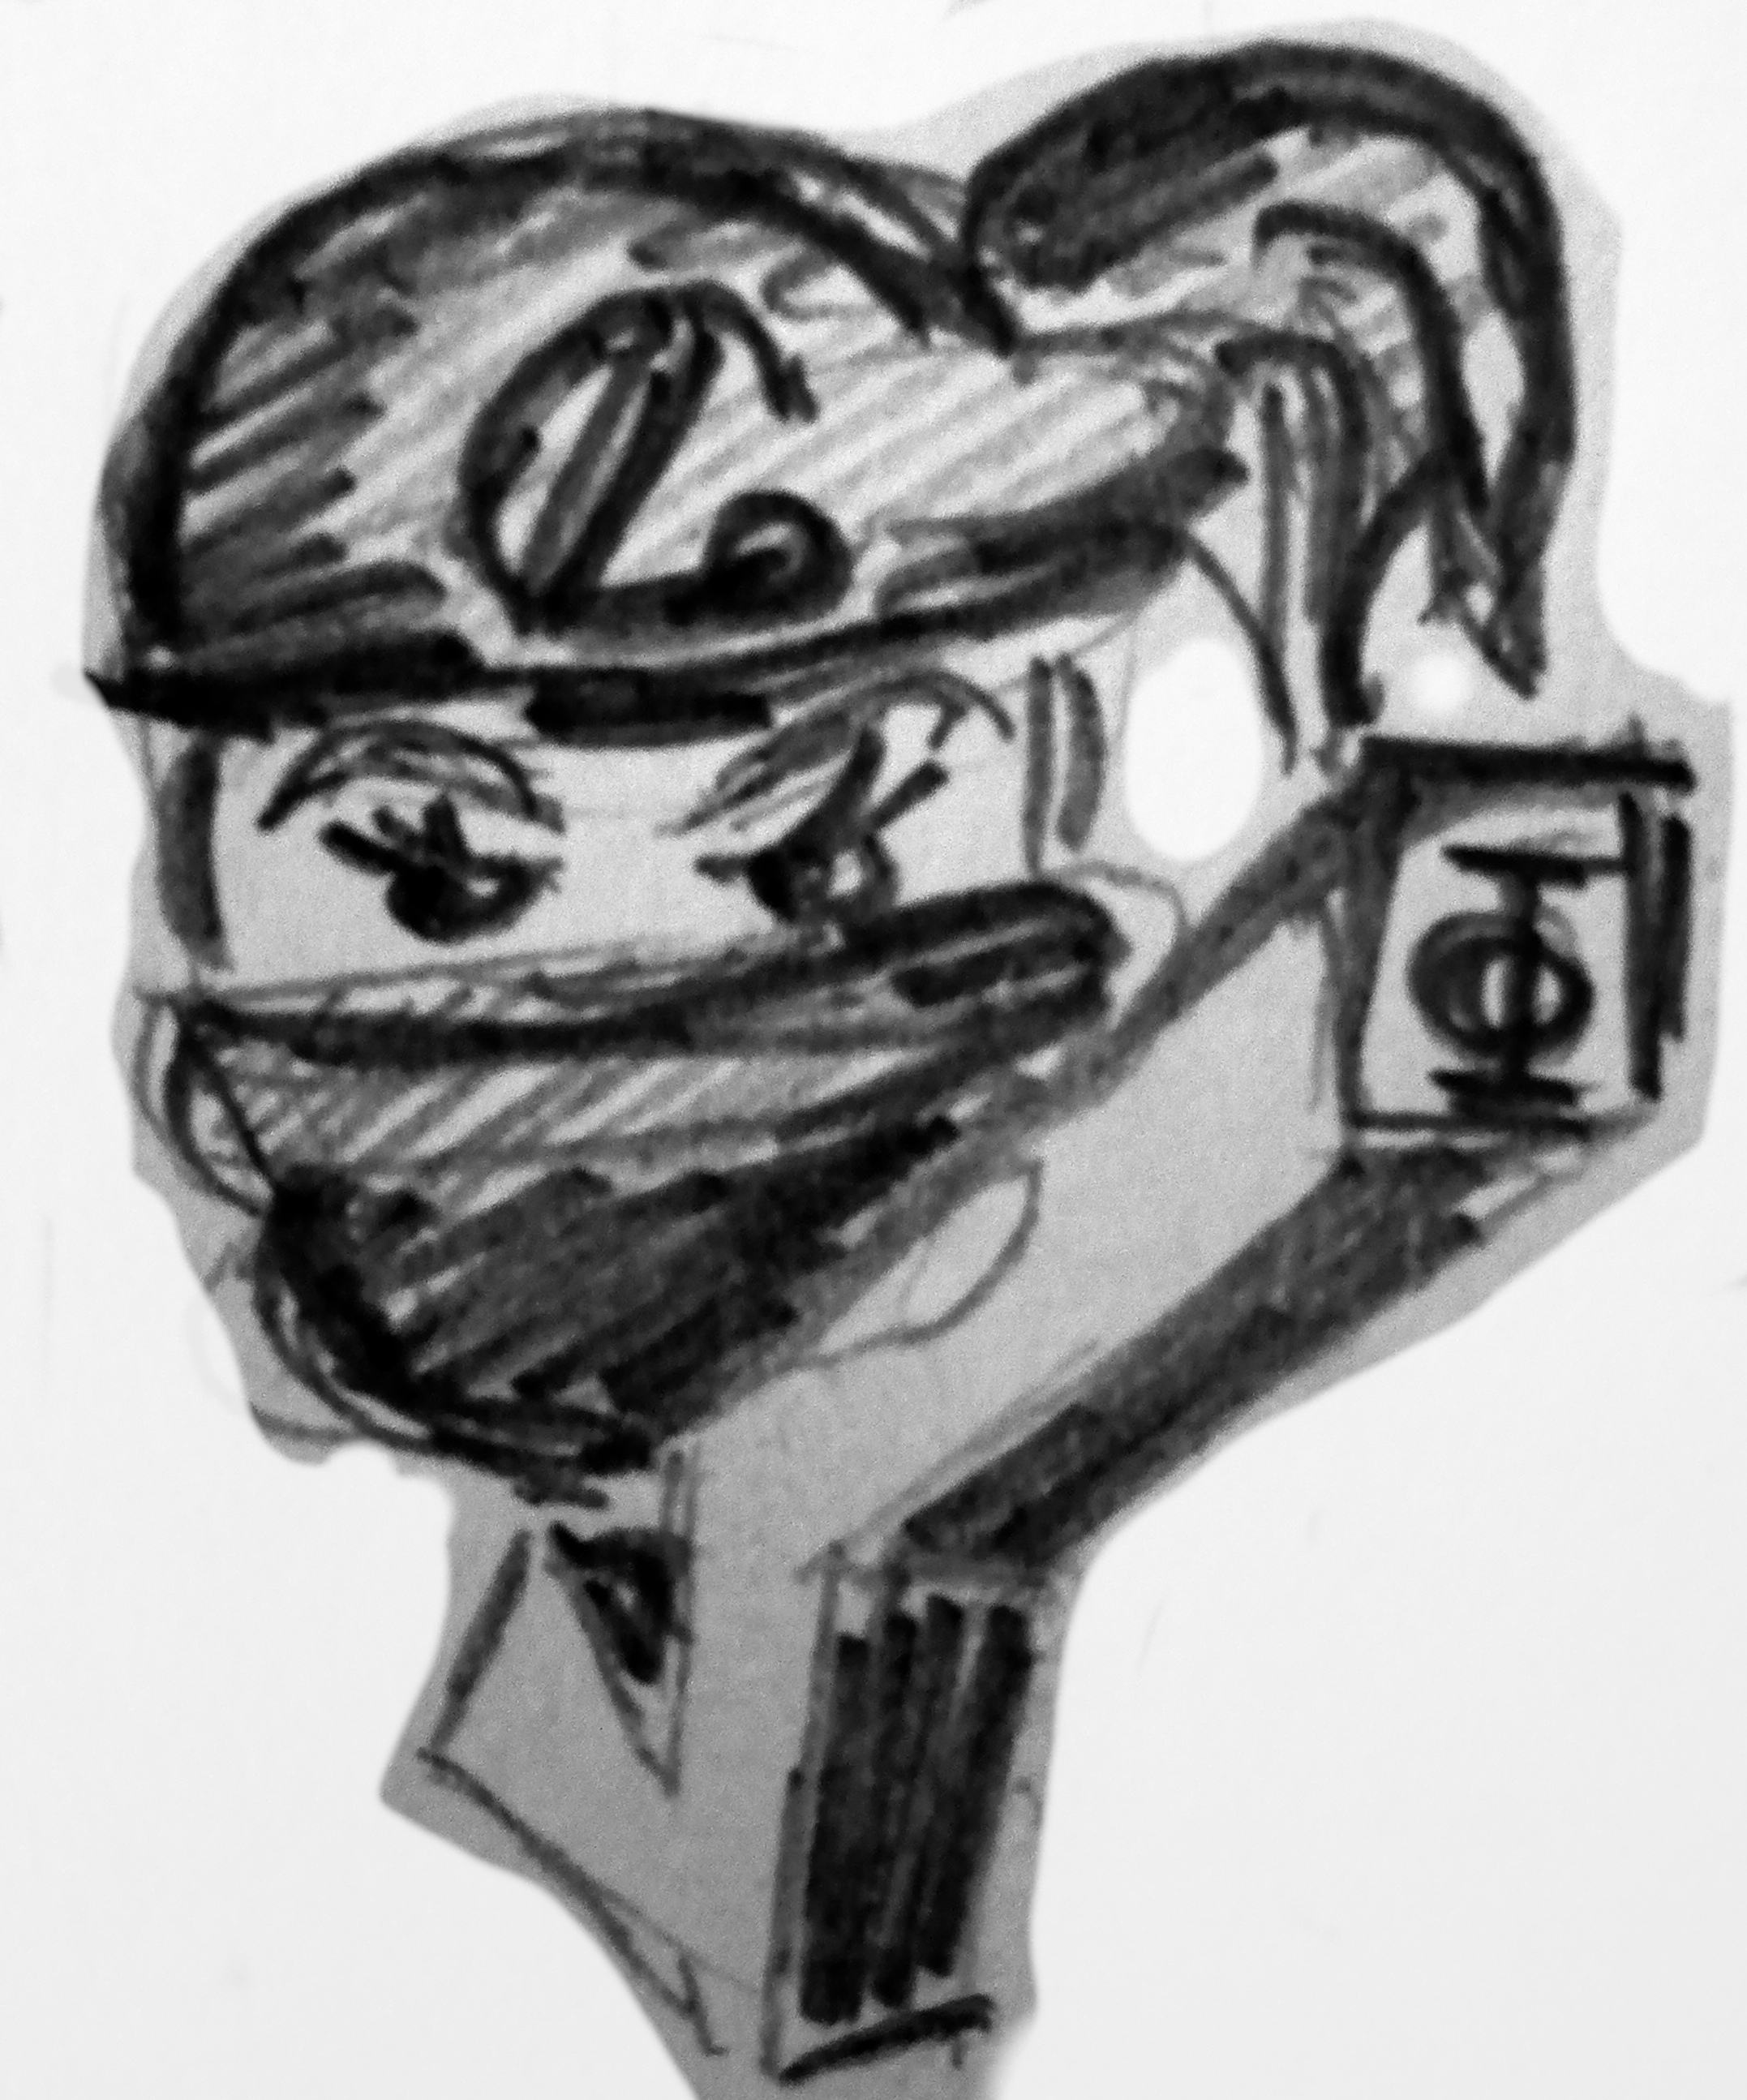
\includegraphics[width=17mm]{img/matheninja/matheninja.jpg}}}{#2}{#1}}

%%\newcommand{\matheNinjaLink}[2]{%%
%%\begin{tabular}{cc}%%
%% \raisebox{-1cm}{
\includegraphics[height=2cm]{img/matheninja/turtle.png}}& \href{#2}{MatheNinja: #1}\\%%
%% \end{tabular}%%
%%}%% End Command  \matheNinjaLink



%% AadB = Aufgaben aus dem Buch
%% 1. Parameter: Seitenzahl
%% 2. Parameter: Aufgabennummern.
%% bsp  \TALSAadB{38-39}{101a-101c, 102 und 103}



%%\newcommand*{\maturaAufgaben}[1]{\begin{mdframed}[backgroundcolor=maturaAufgabenFarbe!10]{#1}\end{mdframed}}

\newcommand*{\aadB}{Aufgaben aus dem Buch}

\newcommand*{\TALSAadB}[2]{%%
{%%
\ifisTALS{\aufgabenFarbe{\noindent{\aadB \cite{frommenwiler17alg}: Seite {#1} Nr. {#2}}}}%%
\fi%%
}}%%

\newcommand*{\TALSGeomAadB}[2]{%%
{%%
\ifisTALS{\aufgabenFarbe{\noindent{\aadB \cite{frommenwiler18geom}: Seite {#1} Nr. {#2}}}}%%
\fi%%
}}%%

\newcommand*{\GESOAadB}[2]{%%
{%%
\ifisGESO{\aufgabenFarbe{\aadB \cite{marthaler21}: Seite {#1} Nr. {#2}}}%%
\fi%%
}}%%

\newcommand*{\theorieGESO}[2]{%%
{\ifisGESO{Theorie \cite{marthaler21}: Seite {#1} Kap. {#2}}%%
\fi%%
}}%%

\newcommand*{\theorieTALS}[2]{%%
{\ifisTALS{Theorie \cite{frommenwiler17alg}: Seite {#1} Kap. {#2}}%%
\fi%%
}}%%

\newcommand*{\theorieTALSGeom}[2]{%%
{\ifisTALS{Theorie \cite{frommenwiler18geom}: Seite {#1} Kap. {#2}}%%
\fi%%
}}%%



%% Referenzen auf Labels
%% AllInOne ist wichtig, denn einige Referenzen funkitionieren nicht
%% in den Themen-Skripts, sondern lediglich in den gesamten Jahres-Skripts.
\newcommand*\totalref[1]{\ifisALLINONE{ (s.\kern 0.22em{}Kap. \ref{#1}
    auf Seite \pageref{#1}) }\else{}\fi{}}%%
\newcommand*\totalrefanhang[1]{ (s.\kern 0.22em{}Kap. \ref{#1}
    auf Seite \pageref{#1}) }%%

%% Short version
\newcommand*\totalrefs[1]{\ifisALLINONE{ Kap. \ref{#1} auf Seite
\pageref{#1} }\else{}\fi{}}%%
%%\newcommand*\aufgabenref[1]{(s\kern 0.22em{}Aufg. \ref{#1} auf Seite \pageref{#1})}

%%%%%%%%%%%%%%%%%%%%%%%%%%%%%%%%%%% BBW Makros %%%%%%%%%%%%%%%%%%%%%%%%%%%%%

